
\documentclass[10pt,stdletter,dateno,sigleft]{newlfm}
\usepackage{pdfpages}
\usepackage{charter} % Use the Charter font for the document text

\newsavebox{\Luiuc}\sbox{\Luiuc}{\parbox[b]{1.75in}{\vspace{0.5in}
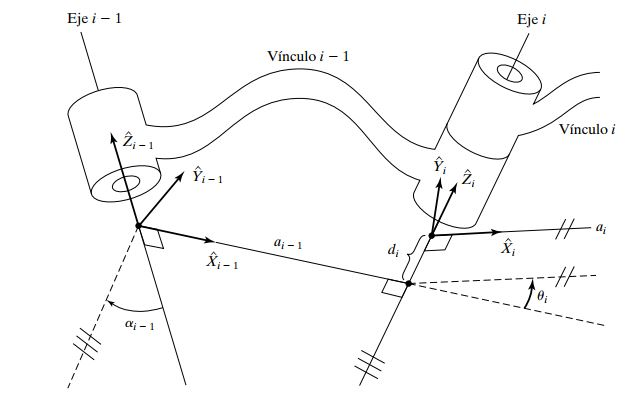
\includegraphics[width=1.2\linewidth]{22.JPG}}} % LOGOTIPO DE LA EMPRESA EN LA PARTE SUPERIOR IZQUIERDA
\makeletterhead{Uiuc}{\Lheader{\usebox{\Luiuc}}}

\newlfmP{sigsize=50pt} % DISMINULLE EL CAMPO DE FIRMA

\lthUiuc % MUESTRA EL LOGO DE LA CNC logo

%----------------------------------------------------------------------------------------
%	YOUR NAME AND CONTACT INFORMATION
%----------------------------------------------------------------------------------------

\namefrom{Everardo Estrella} % Name

\addrfrom{
\date\\[04 de Octubre del 2019] % Date
 \\ % Address
Matricez y desplazamientos
}

%----------------------------------------------------------------------------------------
%	ADDRESSEE AND GREETING/CLOSING
%----------------------------------------------------------------------------------------

\greetto{Desarrollo de un Robot serial del tipo CNC,} 
\closeline{simulacion de Cinematica Directa e Inversa de manipuladores Seriales y sus Singularidades.}

\nameto{Everardo Estrella Rojo} 

\addrto{
Ingeneria en Mecatronica \\ 
Universidad Politecnica \\
Practica 4 \\
Cinematica de Robots
}

%----------------------------------------------------------------------------------------

\begin{document}
\date{FECHA 2019}
\begin{newlfm}

%----------------------------------------------------------------------------------------
%	LETTER CONTENT
%----------------------------------------------------------------------------------------
Parámetros de vínculo
Cualquier robot puede describirse en forma cinemática proporcionando los valores de cuatro cantidades para cada vínculo. Dos describen el vínculo en sí, y los otros dos describen la conexión del vínculo con un vínculo adyacente. En el caso de una articulación angular, θi se llama variable de articulación y las otras tres cantidades son parámetros de vínculo fijos. Para las articulaciones prismáticas, di es la variable de articulación y las otras tres cantidades son parámetros de vínculo fijos. La definición de mecanismos por medio de estas cantidades es una convención que generalmente se le conoce como notación Denavit-Hartenberg
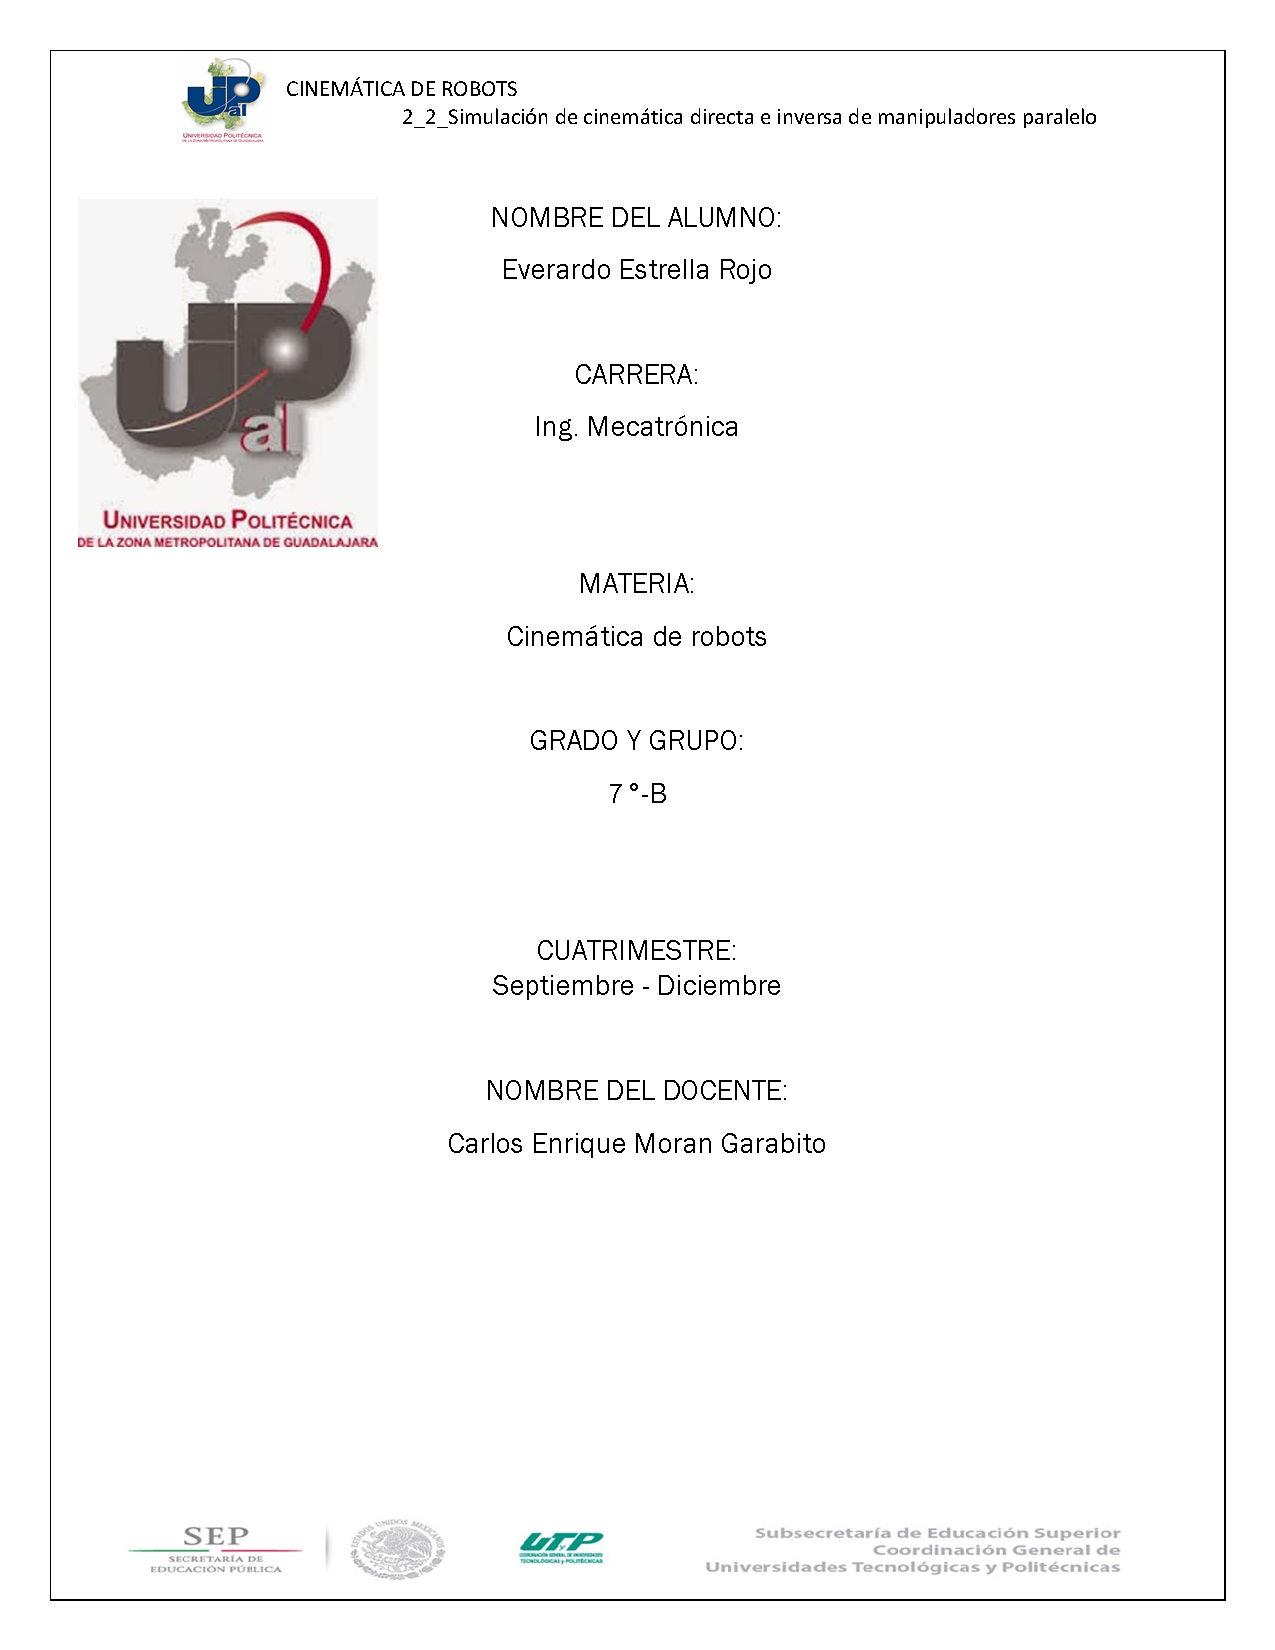
\includepdf[pages=-]{22S}
 

%----------------------------------------------------------------------------------------

\end{newlfm}

\end{document}